\documentclass[11pt, aspectratio=169]{beamer}
\usetheme{default}
\usecolortheme{default}
\setbeamertemplate{navigation symbols}{}
\usepackage{amsmath, amssymb}
\usepackage{booktabs}
\usepackage{tikz}
\usetikzlibrary{trees, patterns, shapes.geometric, arrows.meta, positioning}

\usepackage{iftex}
\ifPDFTeX
  \usepackage[T1]{fontenc}
  \usepackage[utf8]{inputenc}
  \usepackage{lmodern}
\else
  \usepackage{fontspec}
  \usepackage[english]{babel}
  \babelfont{rm}{Montserrat}
  \babelfont{sf}{Lato}
\fi

% --- Corporate Academic Color Palette ---
\definecolor{NavyBlue}{RGB}{24, 43, 73}
\definecolor{AccentBlue}{RGB}{0, 114, 206}
\definecolor{DarkSlate}{RGB}{51, 65, 85}
\definecolor{MutedGray}{RGB}{100, 116, 139}
\definecolor{LightBg}{RGB}{248, 250, 252}
\definecolor{CardBg}{RGB}{241, 245, 249}
\definecolor{SuccessGreen}{RGB}{22, 101, 52}
\definecolor{LeafBg}{RGB}{220, 252, 231}
\definecolor{AlertRed}{RGB}{185, 28, 28}
\definecolor{AlertBg}{RGB}{254, 242, 242}
\definecolor{SoftBlue}{RGB}{224, 242, 254}

% --- Global Colors Configuration ---
\setbeamercolor{background canvas}{bg=LightBg}
\setbeamercolor{normal text}{fg=DarkSlate}
\setbeamercolor{frametitle}{fg=NavyBlue, bg=LightBg}
\setbeamercolor{title}{fg=NavyBlue}
\setbeamercolor{subtitle}{fg=AccentBlue}
\setbeamercolor{author}{fg=DarkSlate}
\setbeamercolor{date}{fg=DarkSlate}
\setbeamercolor{structure}{fg=AccentBlue}

% --- Block Styling ---
\setbeamertemplate{blocks}[rounded][shadow=false]
\setbeamercolor{block title}{bg=NavyBlue, fg=white}
\setbeamercolor{block body}{bg=CardBg, fg=DarkSlate}
\setbeamercolor{block title alerted}{bg=AlertRed, fg=white}
\setbeamercolor{block body alerted}{bg=AlertBg, fg=DarkSlate}
\setbeamercolor{block title example}{bg=AccentBlue, fg=white}
\setbeamercolor{block body example}{bg=blue!6, fg=DarkSlate}

% ==============================================================================
% STANDARD TOP BEAM (HEADLINE)
% ==============================================================================
\setbeamertemplate{headline}{
  \ifnum\insertpagenumber>1
    \begin{beamercolorbox}[wd=\paperwidth,ht=3ex,dp=1.1ex,leftskip=0.8cm,rightskip=0.8cm]{headline}
      {\tiny\bfseries\color{white} ED547: Big Data Analytics \hfill Automated Early Detection of Adverse Drug Interactions}
    \end{beamercolorbox}
    \vspace{-1pt}
    {\color{AccentBlue}\rule{\paperwidth}{1.5pt}}
  \fi
}
\setbeamercolor{headline}{bg=NavyBlue}

% --- Frame Title Customization (Clean, single accent line) ---
\setbeamertemplate{frametitle}{
    \vspace{0.25cm}
    {\normalsize\bfseries\color{NavyBlue}\insertframetitle}
    \par\vspace{0.05cm}
}
\setbeamertemplate{footline}[page number]

% --- Itemize Customization ---
\setbeamertemplate{itemize item}{\color{AccentBlue}$\blacktriangleright$}
\setbeamertemplate{itemize subitem}{\color{AccentBlue}--}

% --- Presentation Metadata ---
\title[Pharmacovigilance FAERS]{Automated Early Detection of Adverse Drug Interactions}
\subtitle{ED547: Big Data Analytics}
\author{Ashish Ranjan \and Aastha Chhabra}
\date{\today}

\begin{document}

% ==============================================================================
% Title Slide (Guaranteed Centered Box & Symmetric 2 Columns)
% ==============================================================================
\begin{frame}[plain]
    \vfill
    \centering
    {\LARGE \bfseries \color{NavyBlue} Automated Early Detection of Adverse Drug Interactions} \\[0.25cm]
    {\normalsize \bfseries \color{AccentBlue} A Distributed Pharmacovigilance Big Data Analytics Pipeline on FDA FAERS} \\[0.55cm]
    
    % Centering wrapper ensuring exact horizontal middle alignment
    \begin{columns}[c]
        \begin{column}{0.84\textwidth}
            \begin{beamercolorbox}[wd=\linewidth,rounded=true,center,sep=8pt]{block body}
                \scriptsize \textbf{\color{NavyBlue}PROJECT CONTRIBUTORS}\\[0.2cm]
                \centering
                \footnotesize
                \begin{tabular}{c@{\hspace{1.8cm}}c}
                     \textbf{Ashish Ranjan} & \textbf{Aastha Chhabra} \\
                     \scriptsize \texttt{IED/10004/22} & \scriptsize \texttt{IED/10005/22}
                \end{tabular}
            \end{beamercolorbox}
        \end{column}
    \end{columns}
    
    \vspace{0.55cm}
    {\footnotesize \color{DarkSlate} Department of Engineering Design \hfill \today}
    \vfill
\end{frame}

% ==============================================================================
% Slide 1: Introduction, Clinical Motive & Big Data Paradigm
% ==============================================================================
\begin{frame}{Introduction, Clinical Motivation \& Big Data Paradigm}
    \begin{columns}[T]
        \begin{column}{0.48\textwidth}
            \begin{block}{\footnotesize 1. Introduction \& FAERS Corpus}
                \begin{itemize}\scriptsize
                    \item \textbf{Pharmacovigilance:} Systematic post-approval surveillance to detect unknown or rare adverse drug reactions.
                    \item \textbf{FDA FAERS System:} $>16\text{M}$ global spontaneous reports from physicians, consumers, and manufacturers.
                \end{itemize}
            \end{block}
            
            \vspace{0.02cm}
            \begin{alertblock}{\footnotesize 2. Clinical Motivation}
                \begin{itemize}\scriptsize
                    \item \textbf{Mortality \& Cost:} Adverse Drug Events (ADEs) are the \textbf{4th leading cause of death} in US hospitals ($>100\text{K}$ deaths/yr, $>\$136\text{B}$ cost).
                    \item \textbf{Trial Limitations:} Pre-market trials ($1\text{K}$--$3\text{K}$ patients) miss rare toxicities ($<1:10,000$), drug interactions (DDIs), and vulnerable cohorts.
                \end{itemize}
            \end{alertblock}
        \end{column}

        \begin{column}{0.48\textwidth}
            \begin{exampleblock}{\footnotesize 3. How Big Data is Leveraged}
                \begin{itemize}\scriptsize
                    \item \textbf{Combinatorial Scale:} Multi-drug regimens $\times$ tens of thousands of reactions across $16\text{M}$ reports cause Out-of-Memory faults in single-node Pandas.
                    \item \textbf{Distributed PySpark:} Vectorized Catalyst optimizer parses nested schemas, deduplicates windowed records, and computes whole-corpus matrices.
                    \item \textbf{Dual Persistence:} Columnar Snappy Parquet on \textbf{Hive} for OLAP; indexed BSON on \textbf{MongoDB} for sub-50ms clinical lookups.
                    \item \textbf{Streaming Telemetry:} Partitioned \textbf{Kafka} topics feed Spark Structured Streaming for prospective, continuous ADE triage.
                \end{itemize}
            \end{exampleblock}
        \end{column}
    \end{columns}
\end{frame}

% ==============================================================================
% Slide 2: End-to-End System Architecture
% ==============================================================================
\begin{frame}{High-Level System Architecture}
    \footnotesize
    \textbf{Architecture Paradigm:} Distributed Decoupled Lakehouse with Real-Time Event Streaming \& Low-Latency Serving.
    \vspace{0.06cm}
    \centering
    \resizebox{0.98\linewidth}{!}{%
    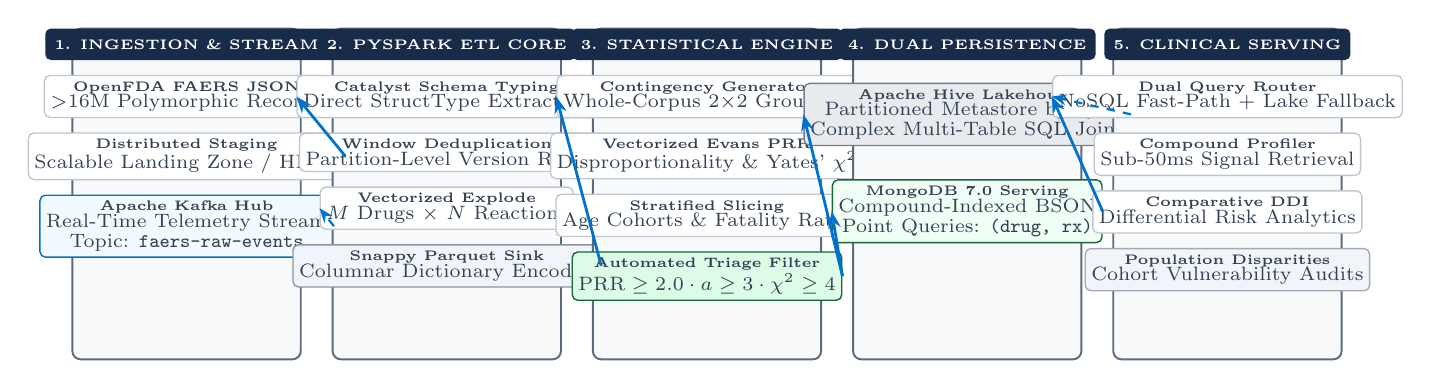
\begin{tikzpicture}[
        node distance=0.18cm,
        layer/.style={rectangle, draw=NavyBlue!70, fill=CardBg!60, rounded corners=3pt, line width=0.7pt, inner sep=3pt},
        header/.style={rectangle, fill=NavyBlue, text=white, font=\tiny\bfseries, rounded corners=2pt, minimum width=2.8cm, minimum height=0.40cm, align=center},
        subnode/.style={rectangle, draw=MutedGray!40, fill=white, rounded corners=2pt, font=\tiny, align=center, inner sep=2.2pt, text=DarkSlate, minimum width=2.7cm, line width=0.5pt},
        flowarr/.style={-{Stealth[scale=0.8]}, draw=AccentBlue, line width=1.0pt},
        dasharr/.style={-{Stealth[scale=0.8]}, draw=AccentBlue, line width=0.8pt, dashed}
    ]
        % Layer 1: Ingestion & Streaming Layer
        \node[layer, minimum width=2.9cm, minimum height=4.2cm] (s1) at (0,0) {};
        \node[header] (h1) at (s1.north) [yshift=-6pt] {1. INGESTION \& STREAM};
        \node[subnode, below=0.18cm of h1] (d1) {\textbf{OpenFDA FAERS JSON}\\\scriptsize $>$16M Polymorphic Records};
        \node[subnode, below=of d1] (raw) {\textbf{Distributed Staging}\\\scriptsize Scalable Landing Zone / HDFS};
        \node[subnode, below=of raw, fill=SoftBlue!40, draw=AccentBlue] (kafka) {\textbf{Apache Kafka Hub}\\\scriptsize Real-Time Telemetry Stream\\\scriptsize Topic: \texttt{faers-raw-events}};

        % Layer 2: Distributed PySpark ETL Engine
        \node[layer, minimum width=2.9cm, minimum height=4.2cm, right=0.38cm of s1] (s2) {};
        \node[header] (h2) at (s2.north) [yshift=-6pt] {2. PYSPARK ETL CORE};
        \node[subnode, below=0.18cm of h2] (ing) {\textbf{Catalyst Schema Typing}\\\scriptsize Direct StructType Extraction};
        \node[subnode, below=of ing] (clean) {\textbf{Window Deduplication}\\\scriptsize Partition-Level Version Rank};
        \node[subnode, below=of clean] (flat) {\textbf{Vectorized Explode}\\\scriptsize $M$ Drugs $\times$ $N$ Reactions};
        \node[subnode, below=of flat, fill=CardBg, draw=NavyBlue!50] (parquet) {\textbf{Snappy Parquet Sink}\\\scriptsize Columnar Dictionary Encoded};

        % Layer 3: Statistical Signal Engine
        \node[layer, minimum width=2.9cm, minimum height=4.2cm, right=0.38cm of s2] (s3) {};
        \node[header] (h3) at (s3.north) [yshift=-6pt] {3. STATISTICAL ENGINE};
        \node[subnode, below=0.18cm of h3] (prrcalc) {\textbf{Contingency Generator}\\\scriptsize Whole-Corpus 2$\times$2 Group-By};
        \node[subnode, below=of prrcalc] (democalc) {\textbf{Vectorized Evans PRR}\\\scriptsize Disproportionality \& Yates' $\chi^2$};
        \node[subnode, below=of democalc] (fatalcalc) {\textbf{Stratified Slicing}\\\scriptsize Age Cohorts \& Fatality Rates};
        \node[subnode, below=of fatalcalc, fill=LeafBg, draw=SuccessGreen] (thresh) {\textbf{Automated Triage Filter}\\\scriptsize $\text{PRR} \ge 2.0 \cdot a \ge 3 \cdot \chi^2 \ge 4$};

        % Layer 4: Dual Persistence Layer
        \node[layer, minimum width=2.9cm, minimum height=4.2cm, right=0.38cm of s3] (s4) {};
        \node[header] (h4) at (s4.north) [yshift=-6pt] {4. DUAL PERSISTENCE};
        \node[subnode, below=0.28cm of h4, fill=NavyBlue!10, draw=NavyBlue!60] (hive) {\textbf{Apache Hive Lakehouse}\\\scriptsize Partitioned Metastore by Qtr\\\scriptsize Complex Multi-Table SQL Joins};
        \node[subnode, below=0.42cm of hive, fill=LeafBg!40, draw=SuccessGreen] (mongo) {\textbf{MongoDB 7.0 Serving}\\\scriptsize Compound-Indexed BSON\\\scriptsize Point Queries: \texttt{(drug, rx)}};

        % Layer 5: Clinical Serving & Analytics UI
        \node[layer, minimum width=2.9cm, minimum height=4.2cm, right=0.38cm of s4] (s5) {};
        \node[header] (h5) at (s5.north) [yshift=-6pt] {5. CLINICAL SERVING};
        \node[subnode, below=0.18cm of h5] (loader) {\textbf{Dual Query Router}\\\scriptsize NoSQL Fast-Path + Lake Fallback};
        \node[subnode, below=of loader] (u1) {\textbf{Compound Profiler}\\\scriptsize Sub-50ms Signal Retrieval};
        \node[subnode, below=of u1] (u2) {\textbf{Comparative DDI}\\\scriptsize Differential Risk Analytics};
        \node[subnode, below=of u2, fill=CardBg, draw=NavyBlue!40] (u3) {\textbf{Population Disparities}\\\scriptsize Cohort Vulnerability Audits};

        % Inter-layer arrows
        \draw[flowarr] (raw.east) -- (ing.west);
        \draw[dasharr] (kafka.east) -- (flat.west);
        \draw[flowarr] (parquet.east) -- (prrcalc.west);
        \draw[flowarr] (thresh.east) -- (hive.west);
        \draw[flowarr] (thresh.east) -- (mongo.west);
        \draw[flowarr] (mongo.east) -- (loader.west);
        \draw[dasharr] (hive.east) -- (loader.west);
    \end{tikzpicture}
    }

    \vspace{0.08cm}
    \begin{beamercolorbox}[wd=0.98\textwidth,rounded=true,center,sep=3pt]{block body}
      \scriptsize \textbf{Big Data Flow:} Raw Multi-Source Telemetry $\longrightarrow$ Distributed PySpark Catalyst ETL $\longrightarrow$ Vectorized Evans Matrix Scoring $\longrightarrow$ Dual Storage (OLAP + NoSQL) $\longrightarrow$ Sub-50ms Clinical Delivery.
    \end{beamercolorbox}
\end{frame}

% ==============================================================================
% Slide 3: Distributed ETL & PySpark Transformations
% ==============================================================================
\begin{frame}[fragile]{Distributed ETL \& Big Data Processing}
    \footnotesize
    \textbf{Engine:} PySpark 3.5.x utilizing pure Columnar DataFrame API with Catalyst query optimization.
    \vspace{0.02cm}
    \begin{columns}[T]
        \begin{column}{0.50\textwidth}
            \begin{block}{\footnotesize Ingestion \& Normalization Stages}
            \begin{enumerate}\scriptsize
                \item \textbf{Schema Parsing:} Reads multi-GB nested JSON via explicit Catalyst Struct schemas without text parsing.
                \item \textbf{Windowed Deduplication:} Retains latest clinical case version:\\
                \texttt{Window.partitionBy("id")}\\
                \texttt{.orderBy(desc("ver"))}
                \item \textbf{Temporal Harmonization:} Standardizes FDA age codes (800--805: Days, Weeks, Months $\to$ Standard Years).
                \item \textbf{Array Explosion:} Resolves combinations:\\
                \texttt{explode("drug")} $\times$ \texttt{explode("reaction")}
                \item \textbf{RxNorm Mapping:} Standardizes brand variations to canonical active generic ingredients.
            \end{enumerate}
            \end{block}
        \end{column}

        \begin{column}{0.49\textwidth}
            \begin{exampleblock}{\footnotesize Distributed Transformation Code}
            \fontsize{5.9pt}{7.0pt}\selectfont
\begin{verbatim}
win = Window.partitionBy("safetyreportid") \
            .orderBy(F.col("version").desc())

clean_reports = raw_df \
  .withColumn("rk", F.row_number().over(win)) \
  .filter(F.col("rk") == 1).drop("rk") \
  .withColumn("drug", F.explode("patient.drug")) \
  .withColumn("rx", F.explode("patient.reaction")) \
  .select(
    F.col("safetyreportid").alias("case_id"),
    F.upper(F.trim("drug.medicinalproduct"))
      .alias("drug_name"),
    F.upper(F.trim("rx.reactionmeddrapt"))
      .alias("reaction"),
    normalize_age_udf("patient.patientonsetage",
      "patient.patientonsetageunit").alias("age"),
    map_sex_udf("patient.patientsex").alias("gender"),
    F.col("serious").cast("int").alias("serious"),
    F.col("seriousnessdeath").cast("int").alias("fatal")
  )
clean_reports.write.mode("overwrite") \
  .parquet("data/processed/reports.parquet")
\end{verbatim}
            \end{exampleblock}
        \end{column}
    \end{columns}
\end{frame}

% ==============================================================================
% Slide 4: Statistical Methodology - Evans Disproportionality
% ==============================================================================
\begin{frame}{Statistical Methodology: Evans Disproportionality Analysis}
    \begin{columns}[T]
        \begin{column}{0.49\textwidth}
            \begin{block}{\footnotesize 2$\times$2 Contingency Matrix Formulation}
                \centering\scriptsize
                For Target Drug $D$ and Target Adverse Reaction $R$:
                \vspace{0.03cm}
                \resizebox{0.95\linewidth}{!}{%
                \begin{tabular}{lccc}
                    \toprule
                    \textbf{Stratum} & \textbf{Event $R$} & \textbf{Other ($\neg R$)} & \textbf{Total} \\
                    \midrule
                    \textbf{Target Drug $D$} & \textbf{$a$} & \textbf{$b$} & $a + b$ \\
                    \textbf{Other Drugs ($\neg D$)} & \textbf{$c$} & \textbf{$d$} & $c + d$ \\
                    \midrule
                    \textbf{Population} & $a + c$ & $b + d$ & $N$ \\
                    \bottomrule
                \end{tabular}%
                }
                \vspace{0.03cm}
            \end{block}

            \begin{exampleblock}{\footnotesize Validated Evans Triage Criteria}
                \scriptsize
                Flagged as an active \textbf{Safety Signal} iff:
                \begin{itemize}\scriptsize
                    \item $\mathbf{\text{PRR} \ge 2.0}$ ($2\times$ relative reporting frequency)
                    \item $\mathbf{a \ge 3}$ (Minimum reporting volume to prevent noise)
                    \item $\mathbf{\chi^2 \ge 4.0}$ (Pearson independence with $p < 0.05$)
                \end{itemize}
            \end{exampleblock}
        \end{column}

        \begin{column}{0.49\textwidth}
            \begin{block}{\footnotesize Mathematical Formulations}
                \scriptsize
                \textbf{1. Proportional Reporting Ratio (PRR):}
                \vspace{-0.15cm}
                \[ \text{PRR} = \frac{a / (a + b)}{c / (c + d)} \]
                \textbf{2. 95\% Confidence Interval Band:}
                \vspace{-0.15cm}
                {\scriptsize
                \[ \text{SE}(\ln \text{PRR}) = \sqrt{\frac{1}{a} - \frac{1}{a + b} + \frac{1}{c} - \frac{1}{c + d}} \]
                \[ \text{PRR}_{95\%\text{ CI}} = \exp\left(\ln \text{PRR} \pm 1.96 \cdot \text{SE}\right) \]
                }
                \textbf{3. $\chi^2$ with Yates' Continuity Correction:}
                \vspace{-0.15cm}
                {\scriptsize \[ \chi^2 = \frac{N \left( |a d - b c| - \frac{N}{2} \right)^2}{(a + b)(c + d)(a + c)(b + d)} \]}
            \end{block}
        \end{column}
    \end{columns}
\end{frame}

% ==============================================================================
% Slide 5: Empirical Benchmark - Rosiglitazone Signal
% ==============================================================================
\begin{frame}{Empirical Benchmark: Rosiglitazone Regulatory Signal}
\footnotesize
\begin{columns}[T]
  \begin{column}{0.50\textwidth}
    \begin{block}{\footnotesize Regulatory Benchmark (FDA 2007 Warning)}
      \centering\scriptsize
      \textbf{Drug:} Rosiglitazone (Avandia) \quad \textbf{Event:} Myocardial Infarction
    \end{block}
    \vspace{0.03cm}
    
    \resizebox{\linewidth}{!}{%
    \begin{tabular}{lccc}
      \toprule
      \textbf{Partition} & \textbf{MI ($R$)} & \textbf{Other ($\neg R$)} & \textbf{Total} \\
      \midrule
      \textbf{Rosiglitazone ($D$)} & $\mathbf{a = 450}$ & $\mathbf{b = 4,550}$ & $5,000$ \\
      \textbf{Other Drugs ($\neg D$)} & $\mathbf{c = 500}$ & $\mathbf{d = 109,500}$ & $110,000$ \\
      \midrule
      \textbf{Marginal Total} & $950$ & $114,050$ & $\mathbf{N = 115,000}$ \\
      \bottomrule
    \end{tabular}
    }
    \vspace{0.06cm}
    \begin{beamercolorbox}[wd=\linewidth,rounded=true,sep=4pt]{exampleblock body}
      \scriptsize \textbf{Clinical Reality:} Replicates the historic FDA Black-Box Warning trigger where Rosiglitazone exhibited lethal cardiac disproportionality.
    \end{beamercolorbox}
  \end{column}

  \begin{column}{0.48\textwidth}
    \begin{block}{\footnotesize Quantitative Verification}
      \scriptsize
      \begin{itemize}\scriptsize
        \item \textbf{Drug Incident Rate:} $\frac{a}{a+b} = \frac{450}{5,000} = \mathbf{0.0900} \; (9.00\%)$
        \item \textbf{Background Rate:} $\frac{c}{c+d} = \frac{500}{110,000} = \mathbf{0.0045} \; (0.45\%)$
        \item \textbf{PRR Point Estimate:} $\frac{0.0900}{0.0045} = \mathbf{19.80} \quad (\gg 2.0)$
        \item \textbf{Pearson Chi-Square:} $\chi^2 = \mathbf{3164.2} \gg 4.0 \; (p < 10^{-10})$
        \item \textbf{95\% Confidence Interval:} $[\mathbf{17.48}, \; \mathbf{22.42}]$
      \end{itemize}
    \end{block}
  \end{column}
\end{columns}
\end{frame}

% ==============================================================================
% Slide 6: Dual Storage & Real-Time Event Streaming
% ==============================================================================
\begin{frame}{Dual Persistence Layer \& Event Streaming}
\footnotesize
\begin{columns}[T]
  \begin{column}{0.49\textwidth}
    \begin{block}{\footnotesize 1. Analytical Lakehouse (Apache Hive)}
      \scriptsize
      \begin{itemize}\scriptsize
        \item \textbf{Columnar Parquet:} Dictionary encoding with Snappy ($>4\times$ reduction vs.\ JSON).
        \item \textbf{Metastore Schema:} External tables partitioned by \texttt{quarter} (\texttt{faers\_events}).
        \item \textbf{HiveQL OLAP:} Complex analytical joins across multi-quarter data.
      \end{itemize}
    \end{block}
    \vspace{0.01cm}
    \begin{block}{\footnotesize 2. Low-Latency Serving (MongoDB 7.0)}
      \scriptsize
      \begin{itemize}\scriptsize
        \item \textbf{BSON Documents:} Pre-computed drug risk profiles and signals.
        \item \textbf{Compound Index:} \texttt{(drug\_name, reaction)} with \texttt{prr: -1}.
        \item \textbf{Sub-50ms Latency:} Instant clinician search responses.
      \end{itemize}
    \end{block}
  \end{column}

  \begin{column}{0.49\textwidth}
    \begin{exampleblock}{\footnotesize Real-Time Event Streaming}
      \centering
      \vspace{0.01cm}
      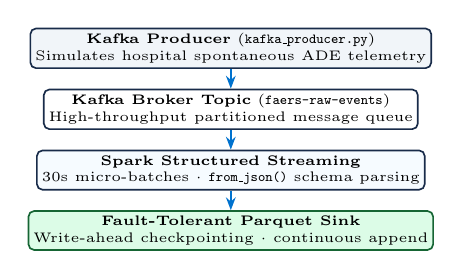
\begin{tikzpicture}[
        node distance=0.25cm,
        stage/.style={rectangle, draw=NavyBlue, fill=white, rounded corners=2pt, font=\tiny, align=center, inner sep=1.8pt, line width=0.6pt, minimum width=3.8cm},
        arr/.style={-{Stealth[scale=0.7]}, draw=AccentBlue, line width=0.8pt}
      ]
        \node[stage, fill=CardBg] (prod) {\textbf{Kafka Producer} (\texttt{kafka\_producer.py})\\\tiny Simulates hospital spontaneous ADE telemetry};
        \node[stage, below=of prod] (topic) {\textbf{Kafka Broker Topic} (\texttt{faers-raw-events})\\\tiny High-throughput partitioned message queue};
        \node[stage, below=of topic, fill=SoftBlue!30] (stream) {\textbf{Spark Structured Streaming}\\\tiny 30s micro-batches $\cdot$ \texttt{from\_json()} schema parsing};
        \node[stage, below=of stream, fill=LeafBg, draw=SuccessGreen] (sink) {\textbf{Fault-Tolerant Parquet Sink}\\\tiny Write-ahead checkpointing $\cdot$ continuous append};

        \draw[arr] (prod) -- (topic);
        \draw[arr] (topic) -- (stream);
        \draw[arr] (stream) -- (sink);
      \end{tikzpicture}
      \vspace{0.01cm}
    \end{exampleblock}
  \end{column}
\end{columns}
\end{frame}

% ==============================================================================
% Slide 7: Real-World Dataset Scale & Volume Reduction
% ==============================================================================
\begin{frame}{Experimental Results: Pipeline Scale \& Data Reduction}
\footnotesize
\begin{columns}[T]
  \begin{column}{0.50\textwidth}
    \begin{block}{\footnotesize Ingested Production Dataset Scale}
      \centering\scriptsize
      \vspace{0.02cm}
      \resizebox{\linewidth}{!}{%
      \begin{tabular}{lrr}
        \toprule
        \textbf{Pipeline Milestone Metric} & \textbf{Count} & \textbf{Scale / State} \\
        \midrule
        Raw Ingested Clinical Cases & $814,596$ & $2.4\text{ GB (JSON)}$ \\
        Clean De-duplicated Reports & $814,596$ & $580\text{ MB (Parquet)}$ \\
        Distinct Active Generic Drugs & $3,412$ & Standardized \\
        Distinct MedDRA Preferred Terms & $11,840$ & Standardized \\
        Evaluated Drug-Reaction Pairs & $110,223$ & Whole Corpus \\
        Validated Evans Safety Signals & $\mathbf{14,892}$ & $\text{PRR} \ge 2.0$ \\
        Critical Lethal Signals ($>20\%$ Fatality) & $\mathbf{1,240}$ & Priority 1 \\
        \bottomrule
      \end{tabular}%
      }
      \vspace{0.02cm}
    \end{block}

    \vspace{0.04cm}
    \begin{beamercolorbox}[wd=\linewidth,rounded=true,sep=3.5pt]{block body}
      \scriptsize \textbf{Data Reduction:} Vectorized aggregation eliminates $>98\%$ irrelevant background combinations into actionable clinical pairs.
    \end{beamercolorbox}
  \end{column}

  \begin{column}{0.48\textwidth}
    \begin{exampleblock}{\footnotesize Volume Funnel \& Compression Ratio}
      \centering
      \vspace{0.03cm}
      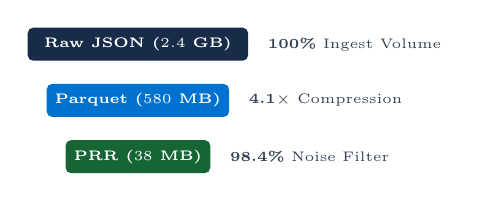
\begin{tikzpicture}[
        bar/.style={rectangle, rounded corners=2pt, font=\tiny\bfseries, align=center, inner sep=3pt, text=white},
        lbl/.style={font=\tiny, text=DarkSlate, anchor=west}
      ]
        \node[bar, fill=NavyBlue, minimum width=2.8cm, minimum height=0.42cm] (b1) {Raw JSON ($2.4\text{ GB}$)};
        \node[bar, fill=AccentBlue, minimum width=1.9cm, minimum height=0.42cm, below=0.28cm of b1] (b2) {Parquet ($580\text{ MB}$)};
        \node[bar, fill=SuccessGreen, minimum width=1.1cm, minimum height=0.42cm, below=0.28cm of b2] (b3) {PRR ($38\text{ MB}$)};

        \node[lbl, right=0.12cm of b1] {\textbf{100\%} Ingest Volume};
        \node[lbl, right=0.12cm of b2] {\textbf{4.1$\times$} Compression};
        \node[lbl, right=0.12cm of b3] {\textbf{98.4\%} Noise Filter};
      \end{tikzpicture}
      \vspace{0.03cm}
    \end{exampleblock}

    \vspace{0.04cm}
    \begin{block}{\footnotesize Computational Throughput \& Serving}
      \scriptsize
      \begin{itemize}\scriptsize
        \item \textbf{Spark Processing:} 4.2 min full-batch ingestion \& 2$\times$2 contingency matrix build across $814\text{K}$ cases.
        \item \textbf{Serving Query Latency:} Indexed MongoDB provides sub-50ms signal lookup for clinicians.
      \end{itemize}
    \end{block}
  \end{column}
\end{columns}
\end{frame}

% ==============================================================================
% Slide 8: Interactive Clinical Dashboard
% ==============================================================================
\begin{frame}{Interactive Clinical Surveillance Platform}
\scriptsize
\centering
\resizebox{0.98\textwidth}{!}{%
\begin{tabular}{lp{10cm}}
  \toprule
  \textbf{Dashboard Domain Module} & \textbf{Clinical Surveillance Functionality \& Visual Analytics} \\
  \midrule
  \textbf{Executive Overview (\texttt{app.py})} & Real-time telemetry monitoring 814,596 patient reports, 110,223 scored pairs, system health badges, and methodology primers. \\
  \textbf{Compound Surveillance (\texttt{01\_drug\_search.py})} & Sub-second query by active pharmaceutical ingredient; computes Evans PRR, 95\% CI, case fatality rates, and demographic distributions. \\
  \textbf{Comparative Profiling (\texttt{02\_drug\_compare.py})} & Head-to-head differential risk ratio ($>1.5\times$) identifying shared adverse reaction disproportionalities between two competing medications. \\
  \textbf{Signal Triage Registry (\texttt{03\_top\_signals.py})} & Multi-factor global prioritization matrix sorting emerging safety signals by PRR score, co-occurrence volume, and case fatality threshold. \\
  \textbf{Population Disparity Audit (\texttt{04\_demographics.py})} & Stratified vulnerability analysis detecting surveillance blind spots across Pediatric (0--17), Adult (18--64), and Geriatric (65+) cohorts. \\
  \bottomrule
\end{tabular}
}

\vspace{0.15cm}
\begin{beamercolorbox}[wd=0.98\textwidth,rounded=true,center,sep=4pt]{block body}
  \scriptsize \textbf{Design System:} Institutional healthcare styling (Inter typography, clinical slate palette, zero emojis, high-contrast Plotly charts).
\end{beamercolorbox}
\end{frame}

% ==============================================================================
% Slide 9: Conclusion & Engineering Merits
% ==============================================================================
\begin{frame}{Conclusion \& Engineering Merits}
\footnotesize
\begin{columns}[T]
  \begin{column}{0.54\textwidth}
    \begin{block}{\footnotesize Engineering Achievements}
      \begin{itemize}\scriptsize
        \item \textbf{Scalable Big Data Core:} PySpark eliminates combinatorial memory bottlenecks across $>16\text{M}$ record schemas.
        \item \textbf{Epidemiological Rigor:} Mathematical Evans PRR with Yates' $\chi^2$ detects genuine safety signals.
        \item \textbf{Dual Architecture:} Columnar Hive lakehouse paired with indexed MongoDB for sub-50ms queries.
        \item \textbf{Real-Time Stream:} Apache Kafka with Spark Streaming enables continuous post-marketing surveillance.
      \end{itemize}
    \end{block}

    \vspace{0.01cm}
    \begin{alertblock}{\footnotesize Production Impact}
      \scriptsize
      Transitions pharmacovigilance from slow, retrospective manual inquiry to automated, real-time prospective safety signal detection.
    \end{alertblock}
  \end{column}

  \begin{column}{0.44\textwidth}
    \begin{exampleblock}{\footnotesize Production Technology Integration}
      \centering
      \vspace{0.01cm}
      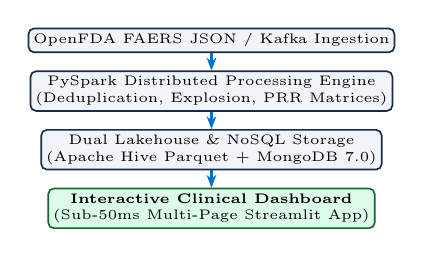
\begin{tikzpicture}[
        node distance=0.22cm,
        stage/.style={rectangle, draw=NavyBlue, fill=CardBg, rounded corners=2pt, font=\tiny, align=center, inner sep=1.8pt, line width=0.6pt, minimum width=3.8cm},
        arr/.style={-{Stealth[scale=0.7]}, draw=AccentBlue, line width=0.8pt}
      ]
        \node[stage] (raw) {OpenFDA FAERS JSON / Kafka Ingestion};
        \node[stage, below=of raw] (spark) {PySpark Distributed Processing Engine\\\tiny (Deduplication, Explosion, PRR Matrices)};
        \node[stage, below=of spark] (store) {Dual Lakehouse \& NoSQL Storage\\\tiny (Apache Hive Parquet + MongoDB 7.0)};
        \node[stage, below=of store, fill=LeafBg, draw=SuccessGreen] (ui) {\textbf{Interactive Clinical Dashboard}\\\tiny (Sub-50ms Multi-Page Streamlit App)};

        \draw[arr] (raw) -- (spark);
        \draw[arr] (spark) -- (store);
        \draw[arr] (store) -- (ui);
      \end{tikzpicture}
      \vspace{0.01cm}
    \end{exampleblock}
  \end{column}
\end{columns}
\end{frame}

\end{document}
